\section{N-Version Programmierung}
\subsection{Definition}
%
%
\begin{frame}
	\frametitle{Überblick}
	\tableofcontents[currentsubsection]
\end{frame}
%
%
\begin{frame}
	\frametitle{N-Version Programmierung - Definition}
	\begin{block}{Definition: N-Version Programmierung \cite{Chen1978}}
		\enquote{\emph{N-version programming is defined as the independent generation of $ N \geq 2 $ functionally equivalent programs, called \enquote{versions}, from the same initial specification.}}
	\end{block}
\end{frame}
%
\subsection{Konzepte}
%
%
\begin{frame}
	\frametitle{Überblick}
	\tableofcontents[currentsubsection]
\end{frame}
%
%
\begin{frame}
	\frametitle{Prinzip}
	Nebenläufige Berechnung der Ergebnisse der N-Versionen und nachfolgender Vergleich um korrektes Ergebnis zu erzielen:
	\begin{figure}
		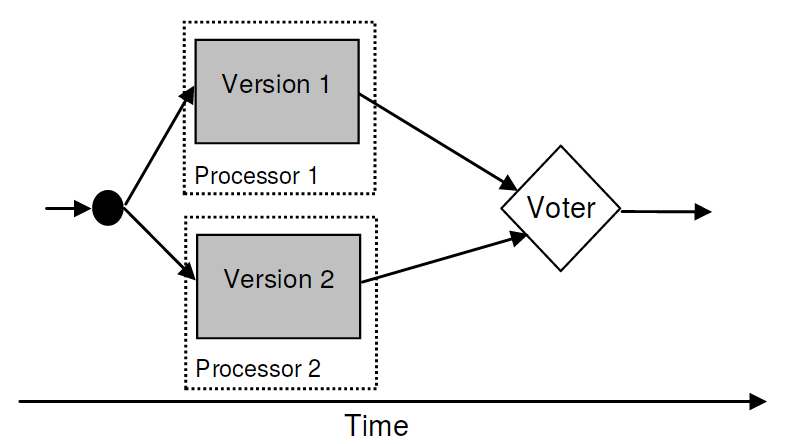
\includegraphics[scale=0.3]{grafiken/multi-thread-n-version.png}		
		\caption{N-Version Software-Unit im Falle von Multi-Threading
			\footnotemark		
		}		
	\end{figure}
	\footnotetext{Quelle: \cite{lucent}}
\end{frame}
%
%
\begin{frame}
	\frametitle{Entwurf - Besondere Komponenten}
	Besondere Komponenten einer N-Version Software-Unit
	\begin{itemize}
		\item Vergleichsvektoren
		\begin{itemize}
			\item Zustand der jeweiligen Version
			\item Variablen, Ereignisse...
		\end{itemize}
		\pause
		\item Vergleichsindikatoren
		\begin{itemize}
			\item Ausgang eines Vergleichs
			\item Anzustoßende Aktion
		\end{itemize}
		\pause
		\item Synchronisationsmechanismen
		\begin{itemize}
			\item Signale zwischen Versionen und Treiber
		\end{itemize}
	\end{itemize}
\end{frame}
%
%
\begin{frame}
	\frametitle{Entwurf - Spezifikation}
	Aufstellen der gemeinsamen Spezifikation:
	\begin{itemize}
		\item Zu implementierende Funktion
		\item Datenformat der Vergleichsvektoren
		\item Zu verwendende Vergleichsalgorithmus
		\item Auf Ausgänge der Vergleiche folgende Aktionen
	\end{itemize}
\end{frame}
%
%
\begin{frame}
	\frametitle{Entwurf - Diversität}
	Diversität in den einzelnen Versionen durch unterschiedliche
	\begin{itemize}
		\item Entwicklerteams
		\item Programmiersprachen
		\item Algorithmen
		\item Compiler
		\item Plattformen
		\item ...
	\end{itemize}
	$\implies$ je unterschiedlicher die Versionen, desto besser.
\end{frame}
%
%
\begin{frame}
	\frametitle{Annahmen über N-Version Programmierung}
	Annahmen der Gründungsväter:
	\begin{itemize}		
		\item Spezifikation als entscheidende Komponente		
		\item Korrektheitsbeweis der Spezifikation günstiger als Beweise einer korrekten Implementierung
		\item Unabhängigkeit von Fehlern
	\end{itemize}
\end{frame}
%
%
\begin{frame}
	\frametitle{Tolerierbare Fehler}
	Welche Fehler können toleriert werden?
	\begin{itemize}		
		\item Implementierungsfehler durch unabhängige Entwicklung
		\item Laufzeitumgebungsfehler durch Streuen der Versionen auf verschiedene Plattformen
	\end{itemize}
\end{frame}
%
%
\subsection{Beispiel}
%
\begin{frame}
	\frametitle{Überblick}
	\tableofcontents[currentsubsection]
\end{frame}
%
\begin{frame}
	\frametitle{Beispiel}
	Airbus 320 mit 4 vorhandenen Versionen des Flugkontrollsystems , 2 davon im ständigen Betrieb
	\begin{figure}
		
\includegraphics[scale=0.13]{grafiken/A320_Atlantic_Airways.jpg}		
		\caption{Airbus 320
			\footnotemark		
		}		
	\end{figure}
	\footnotetext{Quelle: \url{airbus.com}}
\end{frame}